% ============================================================
% 00-bezier-overview.tex
% Compile with:  pdflatex -shell-escape 00-bezier-overview.tex
% Run twice for table of contents.
% ============================================================

\documentclass[12pt, a4paper]{article}

\usepackage[T1]{fontenc}
\usepackage[utf8]{inputenc}
\usepackage{lmodern}
\usepackage[top=2.5cm, bottom=2.5cm, left=2.8cm, right=2.8cm]{geometry}
\usepackage[dvipsnames]{xcolor}

\definecolor{codebg}{RGB}{248,248,248}
\definecolor{rulecolor}{RGB}{180,180,180}
\definecolor{examplebg}{RGB}{240,248,255}
\definecolor{examplerule}{RGB}{100,149,237}
\definecolor{notebg}{RGB}{255,250,230}
\definecolor{noterule}{RGB}{210,180,50}
\definecolor{diffbg}{RGB}{240,255,240}
\definecolor{diffrule}{RGB}{80,160,80}
\definecolor{samebg}{RGB}{245,245,245}
\definecolor{samerule}{RGB}{160,160,160}
\definecolor{curvecol}{RGB}{70,130,180}
\definecolor{polycol}{RGB}{220,50,50}
\definecolor{pointcol}{RGB}{34,139,34}
\definecolor{dccol1}{RGB}{255,165,0}
\definecolor{dccol2}{RGB}{148,0,211}

\usepackage{minted}
\setminted[julia]{
  bgcolor=codebg, frame=leftline, framerule=1.5pt,
  rulecolor=rulecolor, linenos=false, fontsize=\small,
  breaklines=true, tabsize=4, style=friendly,
}
\setminted[bash]{
  bgcolor=codebg, frame=leftline, framerule=1.5pt,
  rulecolor=rulecolor, fontsize=\small,
}

\usepackage{amsmath}
\usepackage{amssymb}
\usepackage{tikz}
\usetikzlibrary{shapes.geometric, arrows.meta, positioning,
                decorations.markings, calc}
\usepackage{mdframed}

\newmdenv[backgroundcolor=examplebg, linecolor=examplerule,
  linewidth=1.5pt, leftline=true, rightline=false,
  topline=false, bottomline=false,
  innerleftmargin=10pt, innerrightmargin=8pt,
  innertopmargin=6pt, innerbottommargin=6pt,
  skipabove=6pt, skipbelow=4pt]{examplebox}

\newmdenv[backgroundcolor=notebg, linecolor=noterule,
  linewidth=1.5pt, leftline=true, rightline=false,
  topline=false, bottomline=false,
  innerleftmargin=10pt, innerrightmargin=8pt,
  innertopmargin=6pt, innerbottommargin=6pt,
  skipabove=6pt, skipbelow=4pt]{notebox}

\newmdenv[backgroundcolor=diffbg, linecolor=diffrule,
  linewidth=1.5pt, leftline=true, rightline=false,
  topline=false, bottomline=false,
  innerleftmargin=10pt, innerrightmargin=8pt,
  innertopmargin=6pt, innerbottommargin=6pt,
  skipabove=6pt, skipbelow=4pt]{insightbox}

\newmdenv[backgroundcolor=samebg, linecolor=samerule,
  linewidth=1.5pt, leftline=true, rightline=false,
  topline=false, bottomline=false,
  innerleftmargin=10pt, innerrightmargin=8pt,
  innertopmargin=6pt, innerbottommargin=6pt,
  skipabove=6pt, skipbelow=4pt]{samebox}

\usepackage[colorlinks=true, linkcolor=black, urlcolor=MidnightBlue]{hyperref}
\usepackage{booktabs}
\usepackage{needspace}
\usepackage{parskip}
\usepackage{titlesec}
\usepackage{fancyhdr}
\usepackage{datetime2}
\usepackage{array}
\usepackage{multirow}

\titleformat{\section}
  {\large\bfseries\color{MidnightBlue}}{\thesection.}{0.6em}{}
  [\vspace{-4pt}\rule{\linewidth}{0.4pt}]
\titleformat{\subsection}
  {\normalsize\bfseries\color{BrickRed}}{\thesubsection.}{0.5em}{}
\titleformat{\subsubsection}
  {\normalsize\bfseries}{\thesubsubsection.}{0.5em}{}

\pagestyle{fancy}
\fancyhf{}
\rhead{\textcolor{gray}{\small 00-bezier-overview}}
\lhead{\textcolor{gray}{\small B\'ezier Series --- Overview}}
\cfoot{\thepage}
\renewcommand{\headrulewidth}{0.3pt}

\newcommand{\cd}[1]{\texttt{#1}}

\title{%
  \vspace{1cm}
  {\LARGE\bfseries B\'ezier Curve Series}\\[0.4em]
  {\large Overview and Reader's Guide}\\[0.4em]
  {\normalsize Julia + GLMakie + Symbolics.jl}\\[0.4em]
  {\normalsize\texttt{Scripts 01--35}}
}
\author{E.R.\ Nurwijayadi}
\date{\DTMtoday}

\begin{document}

\maketitle
\thispagestyle{empty}

\begin{center}
\textit{Directed and curated by E.R.\ Nurwijayadi.
Code and explanations AI-generated.}
\end{center}

\vspace{0.5em}
\begin{center}
\begin{minipage}{0.82\textwidth}
\small\itshape
B\'ezier curves are everywhere: the rounded corners of
every app button, the letterforms of every font on your
screen, the smooth swoop of a car body, the easing on
every animation.
You interact with them dozens of times a day without
noticing.

After working through this series, you will notice them
every time --- and know exactly how they work.

Why did the control point feel left out?
Because the curve never passes through it.
(That is the only joke.
Everything that follows is serious.)
\end{minipage}
\end{center}

\vspace{1em}\hrule\vspace{1.5em}
\tableofcontents
\newpage


% =============================================================
\needspace{8\baselineskip}
\section{What Is a B\'ezier Curve?}
% =============================================================

\subsection{The geometric idea}

A B\'ezier curve is a smooth parametric curve defined by
a small set of \textbf{control points}.
The curve passes through the first and last control points
(the endpoints) but is only \emph{attracted} by the
intermediate ones --- it bends toward them without
touching them.

The curve is traced by a parameter $u$ that sweeps from
0 to 1.
At $u = 0$ you are at the first control point.
At $u = 1$ you are at the last.
At every $u$ in between you are somewhere on the smooth
curve connecting them.

\begin{center}
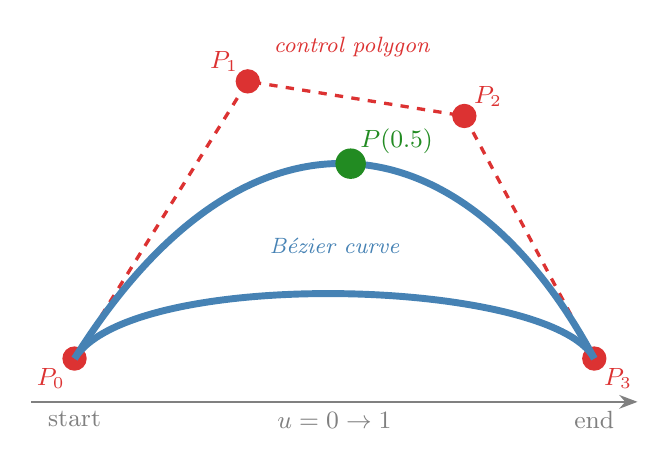
\begin{tikzpicture}[scale=1.1]

  % Control points
  \coordinate (P0) at (0, 0);
  \coordinate (P1) at (2, 3.2);
  \coordinate (P2) at (4.5, 2.8);
  \coordinate (P3) at (6, 0);

  % Control polygon
  \draw[polycol, dashed, line width=1.2pt]
    (P0) -- (P1) -- (P2) -- (P3);

  % Control point markers
  \foreach \p/\lbl/\pos in
    {P0/P_0/below left, P1/P_1/above left,
     P2/P_2/above right, P3/P_3/below right} {
    \fill[polycol] (\p) circle (4pt);
    \node[\pos, polycol, font=\small\bfseries] at (\p)
      {$\lbl$};
  }

  % Bezier curve (cubic, computed via Bernstein)
  \draw[curvecol, line width=2.5pt]
    (P0) .. controls ($(P0)!0.333!(P1)$) and ($(P3)!0.333!(P2)$) .. (P3);

  % Actually draw a proper cubic bezier
  \draw[curvecol, line width=2.5pt]
    (0,0) .. controls (2,3.2) and (4.5,2.8) .. (6,0);

  % Highlighted point at u=0.5
  % cubic bezier at u=0.5: (1-u)^3*P0 + 3u(1-u)^2*P1 + 3u^2(1-u)*P2 + u^3*P3
  % = 0.125*(0,0) + 0.375*(2,3.2) + 0.375*(4.5,2.8) + 0.125*(6,0)
  % = (0,0) + (0.75,1.2) + (1.6875,1.05) + (0.75,0)
  % = (3.1875, 2.25)
  \fill[pointcol] (3.1875, 2.25) circle (5pt);
  \node[above right, pointcol, font=\small]
    at (3.1875, 2.25) {$P(0.5)$};

  % u arrow along curve
  \draw[-Stealth, gray, thick]
    (-0.5, -0.5) -- node[below, font=\small\itshape]{$u = 0 \to 1$}
    (6.5, -0.5);
  \node[below, gray, font=\small] at (0,-0.5) {start};
  \node[below, gray, font=\small] at (6,-0.5) {end};

  % Labels
  \node[font=\footnotesize\itshape, curvecol]
    at (3.0, 1.3) {B\'ezier curve};
  \node[font=\footnotesize\itshape, polycol]
    at (3.2, 3.6) {control polygon};

\end{tikzpicture}
\end{center}

\medskip
The \textbf{control polygon} (dashed red) is the skeleton.
The \textbf{B\'ezier curve} (solid blue) is the smooth result.
The green dot shows the curve point at $u = 0.5$.

\needspace{5\baselineskip}
\subsection{The convex hull property}

Every point on a B\'ezier curve is a weighted average of
the control points, where all weights are non-negative
and sum to 1.
This means the curve is always contained inside the
convex hull of its control points --- the smallest
convex shape that encloses all of them.

This property has a practical consequence: if you move
a control point, only the part of the curve near that
point changes.
The rest is unaffected.

\needspace{5\baselineskip}
\subsection{Degree and number of control points}

\begin{center}
\begin{tabular}{lcll}
\toprule
Name & Degree & Control points & Curve shape \\
\midrule
Linear    & 1 & 2 & Straight line \\
Quadratic & 2 & 3 & Single arc \\
Cubic     & 3 & 4 & S-curve possible \\
Quartic   & 4 & 5 & More complex shapes \\
Degree $n$ & $n$ & $n+1$ & General \\
\bottomrule
\end{tabular}
\end{center}

This series works with quadratic (scripts~11--12) and
quartic (scripts~21--22) as concrete cases, then
generalises to any degree (scripts~31--35).


% =============================================================
\needspace{8\baselineskip}
\section{The Two Evaluation Methods}
% =============================================================

\textit{Given a set of control points and a parameter $u$,
how do you find the point on the curve?
The series explores two methods that always give the same
answer but work in completely different ways.}

\needspace{5\baselineskip}
\subsection{Method 1: Bernstein polynomials}

The Bernstein method computes a weighted average of all
control points simultaneously:
\[
  P(u) = \sum_{i=0}^{n} B(n, i, u) \cdot P_i
  \qquad
  B(n, i, u) = \binom{n}{i} u^i (1-u)^{n-i}
\]

Each $B(n, i, u)$ is a weight that tells you how much
influence control point $P_i$ has at parameter $u$.
All weights are non-negative and sum to 1.
At $u = 0$, only $P_0$ has weight 1; all others are 0.
At $u = 1$, only $P_n$ has weight 1.
In between, the weights blend smoothly.

\begin{examplebox}
\textbf{Quadratic ($n=2$) at $u=0.5$:}

$B(2,0,0.5) = 0.25$, \quad
$B(2,1,0.5) = 0.50$, \quad
$B(2,2,0.5) = 0.25$

$P(0.5) = 0.25 P_0 + 0.50 P_1 + 0.25 P_2$

The midpoint control point $P_1$ contributes twice as
much as the endpoints --- the curve is pulled toward
it, but only reaches halfway.
\end{examplebox}

\needspace{5\baselineskip}
\subsection{Method 2: De Casteljau algorithm}

The De Casteljau method is purely geometric.
Instead of computing weights, it repeatedly cuts line
segments.

At each step, slide fraction $u$ along every edge of
the current polygon to get a new, shorter polygon.
After $n$ steps for a degree-$n$ curve, you are left
with a single point --- the curve point at parameter $u$.

\begin{center}
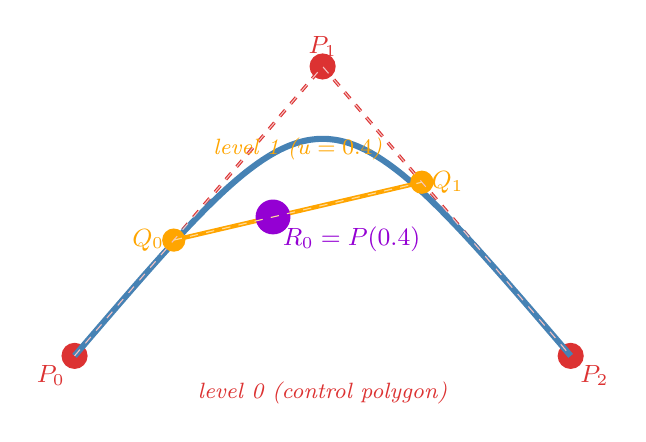
\begin{tikzpicture}[scale=1.05]

  % Control points (quadratic)
  \coordinate (P0) at (0, 0);
  \coordinate (P1) at (3, 3.5);
  \coordinate (P2) at (6, 0);

  % Level 0: control polygon
  \draw[polycol, dashed, line width=1.2pt]
    (P0) -- (P1) -- (P2);
  \foreach \p/\lbl/\pos in
    {P0/P_0/below left, P1/P_1/above, P2/P_2/below right} {
    \fill[polycol] (\p) circle (4.5pt);
    \node[\pos, polycol, font=\small\bfseries] at (\p) {$\lbl$};
  }

  % Bezier curve
  \draw[curvecol, line width=2.2pt]
    (P0) .. controls (P1) .. (P2);

  % Level 1: Q0 and Q1 at u=0.4
  % Q0 = (1-0.4)*P0 + 0.4*P1 = 0.6*(0,0) + 0.4*(3,3.5) = (1.2, 1.4)
  % Q1 = (1-0.4)*P1 + 0.4*P2 = 0.6*(3,3.5) + 0.4*(6,0) = (1.8+2.4, 2.1) = (4.2, 2.1)
  \coordinate (Q0) at (1.2, 1.4);
  \coordinate (Q1) at (4.2, 2.1);

  \draw[dccol1, line width=1.6pt] (Q0) -- (Q1);
  \foreach \p/\lbl/\pos in
    {Q0/Q_0/left, Q1/Q_1/right} {
    \fill[dccol1] (\p) circle (4pt);
    \node[\pos, dccol1, font=\small\bfseries] at (\p) {$\lbl$};
  }

  % Level 2: R0 at u=0.4
  % R0 = (1-0.4)*Q0 + 0.4*Q1 = 0.6*(1.2,1.4) + 0.4*(4.2,2.1)
  %    = (0.72, 0.84) + (1.68, 0.84) = (2.4, 1.68)
  \coordinate (R0) at (2.4, 1.68);
  \fill[dccol2] (R0) circle (6pt);
  \node[below right, dccol2, font=\small\bfseries] at (R0) {$R_0 = P(0.4)$};

  % Connector lines (faint)
  \draw[polycol!30, dashed, thin]
    (P0) -- (Q0) -- (P1) -- (Q1) -- (P2);
  \draw[dccol1!40, dashed, thin]
    (Q0) -- (R0) -- (Q1);

  % Annotations
  \node[font=\footnotesize\itshape, dccol1]
    at (2.7, 2.5) {level 1 ($u=0.4$)};
  \node[font=\footnotesize\itshape, polycol]
    at (3.0, -0.45) {level 0 (control polygon)};

\end{tikzpicture}
\end{center}

\medskip
The orange segment $Q_0Q_1$ is level~1:
each $Q$ point is 40\% of the way along its parent edge.
The purple point $R_0$ is 40\% of the way along $Q_0Q_1$ ---
it sits exactly on the curve.

\needspace{5\baselineskip}
\subsection{Which method does the series use where?}

\begin{center}
\begin{tabular}{lll}
\toprule
Method & Scripts & Why \\
\midrule
Bernstein (algebra) & 01--05 & Exact polynomial form \\
Bernstein (plotting) & 11, 21, 31, 32 & Efficient for many points \\
De Casteljau & 12, 22, 31--35 & Geometric insight, visualisation \\
Both together & 31--35 & Comparison and curvature \\
\bottomrule
\end{tabular}
\end{center}

Both methods are implemented in parallel throughout the
series.
They always produce the same curve --- the series uses
both precisely to demonstrate this equivalence.


% =============================================================
\needspace{8\baselineskip}
\section{The Series at a Glance}
% =============================================================

\subsection{Three groups, one progression}

The 15 scripts fall naturally into three groups:

\begin{center}
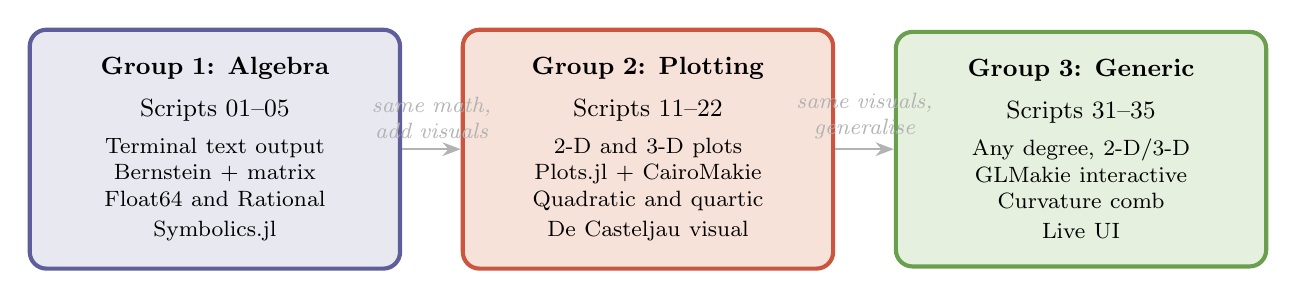
\begin{tikzpicture}[font=\small]

  \tikzset{
    groupbox/.style={rectangle, rounded corners=6pt,
      draw=#1!70, fill=#1!10, line width=1.5pt,
      inner sep=10pt, text width=4cm, align=center},
    arrowstyle/.style={-Stealth, thick, gray!60}
  }

  \node[groupbox=MidnightBlue] (g1) at (0, 0) {
    \textbf{Group 1: Algebra}\\[4pt]
    Scripts 01--05\\[4pt]
    \footnotesize
    Terminal text output\\
    Bernstein + matrix\\
    Float64 and Rational\\
    Symbolics.jl
  };

  \node[groupbox=BrickRed] (g2) at (5.5, 0) {
    \textbf{Group 2: Plotting}\\[4pt]
    Scripts 11--22\\[4pt]
    \footnotesize
    2-D and 3-D plots\\
    Plots.jl + CairoMakie\\
    Quadratic and quartic\\
    De Casteljau visual
  };

  \node[groupbox=OliveGreen] (g3) at (11, 0) {
    \textbf{Group 3: Generic}\\[4pt]
    Scripts 31--35\\[4pt]
    \footnotesize
    Any degree, 2-D/3-D\\
    GLMakie interactive\\
    Curvature comb\\
    Live UI
  };

  \draw[arrowstyle] (g1) -- node[above, font=\footnotesize\itshape,
    text width=2cm, align=center]
    {same math, add visuals} (g2);
  \draw[arrowstyle] (g2) -- node[above, font=\footnotesize\itshape,
    text width=2cm, align=center]
    {same visuals, generalise} (g3);

\end{tikzpicture}
\end{center}

\needspace{5\baselineskip}
\subsection{All 15 scripts}

\begin{center}
\renewcommand{\arraystretch}{1.2}
\begin{tabular}{lp{4.2cm}p{2.2cm}p{3.8cm}}
\toprule
Script & Name & Output & Key new concept \\
\midrule
\rowcolor{examplebg}
01 & bezier-algebra & Text & Hand-rolled \cd{Poly}, multiple dispatch \\
02 & bezier-sympy & Text & \cd{Rational\{Int\}}, Symbolics.jl \\
\rowcolor{examplebg}
03 & bezier-matrix-pedagogical & Text & $U \cdot M \cdot G$, step-by-step \\
04 & bezier-matrix-straight & Text & Section-based output \\
\rowcolor{examplebg}
05 & bezier-matrix-sympy-text & Text & Symbolic + rational combined \\
\midrule
11p & bezier-quadratic-plots & 2-D plot & Plots.jl, \cd{hcat+splat+transpose} \\
\rowcolor{examplebg}
11m & bezier-quadratic-makie & 2-D plot & CairoMakie, Figure/Axis split \\
12p & de-casteljau-plots & 2-D plot & \cd{lerp}, named tuple, snapshots \\
\rowcolor{examplebg}
12m & de-casteljau-makie & 2-D plot & \cd{titlegap}, legend control \\
\midrule
21 & bezier-quartic-makie & 3-D static & \cd{Axis3}, elevation/azimuth \\
\rowcolor{examplebg}
22 & de-casteljau-makie (3D) & 3-D static & \cd{getfield}, NaN dummy lines \\
\midrule
31 & bezier-generic & 2-D/3-D & GLMakie, \cd{is\_3d} branch, generic DC \\
\rowcolor{examplebg}
32 & bezier-symbolic & 2-D/3-D & \cd{build\_symbolic\_poly}, substitution \\
34 & bezier-curvature & 2-D/3-D & Derivative control points, comb \\
\rowcolor{examplebg}
35 & bezier-interactive & UI & \cd{Observable}, sliders, textboxes \\
\bottomrule
\end{tabular}
\end{center}

\begin{notebox}
\textbf{Why is there no script 33?}
The numbering follows the Python source series from which
the Julia scripts were ported.
Script~33 exists in the original series but was not
included here.
\end{notebox}


% =============================================================
\needspace{8\baselineskip}
\section{How to Read These Documents}
% =============================================================

\subsection{Document naming}

Each script has one or more explanation documents.
The naming convention is:

\begin{center}
\begin{tabular}{lp{8.5cm}}
\toprule
Filename pattern & Contents \\
\midrule
\cd{NN-name-code-explained.tex} &
  Code explanation only (scripts 01--05) \\
\cd{NN-name-output-explained.tex} &
  Output explanation only (scripts 01--05) \\
\cd{NN-name-explained.tex} &
  Merged: plot first, then code (scripts 11--35) \\
\cd{40-bezier-code-analysis.tex} &
  Series-wide architecture and pattern analysis \\
\cd{00-bezier-overview.tex} &
  This document \\
\bottomrule
\end{tabular}
\end{center}

\needspace{5\baselineskip}
\subsection{Box colour meanings}

Four coloured boxes appear throughout the documents.
Each has a consistent meaning:

\begin{center}
\begin{tabular}{p{1.8cm}p{3cm}p{7cm}}
\toprule
Colour & Name & Used for \\
\midrule
\cellcolor{examplebg}\textcolor{examplerule}{\rule{6pt}{6pt}}
  Blue &
  Example box &
  Concrete worked examples with actual numbers.
  Traces through what the code computes. \\[6pt]
\cellcolor{notebg}\textcolor{noterule}{\rule{6pt}{6pt}}
  Yellow &
  Note box &
  Warnings, caveats, and ``why'' explanations.
  Things that would bite a beginner. \\[6pt]
\cellcolor{diffbg}\textcolor{diffrule}{\rule{6pt}{6pt}}
  Green &
  Insight box &
  Design insights, patterns, and broader context.
  The bigger picture. \\[6pt]
\cellcolor{samebg}\textcolor{samerule}{\rule{6pt}{6pt}}
  Grey &
  Reference box &
  ``This was explained earlier.''
  Points to the prior document rather than repeating. \\
\bottomrule
\end{tabular}
\end{center}

\needspace{5\baselineskip}
\subsection{Typographic conventions}

\begin{center}
\begin{tabular}{lp{9cm}}
\toprule
Convention & Meaning \\
\midrule
\cd{monospace} & Julia code, function names, variable names,
  type names, filenames \\
$P(u)$, $\kappa$, $u$ & Mathematical quantities \\
\textbf{bold} & First use of an important term \\
\textit{italic} & Emphasis or a note to the reader \\
\bottomrule
\end{tabular}
\end{center}

\needspace{5\baselineskip}
\subsection{Each document is self-contained}

Every explanation document can be read independently.
Where a concept was introduced in a prior script,
a grey reference box points back to it rather than
repeating the full explanation.
This means you can start at any script without having
read all the previous ones --- though of course reading
in order gives the clearest picture.

\needspace{5\baselineskip}
\subsection{Data tables}

The plotting documents (scripts 11--35) include concrete
data tables showing the actual values of key variables
such as the curve matrix \cd{cpts}, the control polygon
matrix \cd{cp}, the highlighted points \cd{hpts},
and the individual point vector \cd{pt}.
These ground the abstract code in real numbers.


% =============================================================
\needspace{8\baselineskip}
\section{Setting Up}
% =============================================================

\subsection{Installing Julia packages}

All required packages must be installed once before
running any script.
Open a Julia REPL and run:

\begin{minted}{julia}
import Pkg; Pkg.add("Symbolics")
import Pkg; Pkg.add("Plots")
import Pkg; Pkg.add("CairoMakie")
import Pkg; Pkg.add("GLMakie")
\end{minted}

\begin{center}
\begin{tabular}{lll}
\toprule
Package & Used in & Purpose \\
\midrule
\cd{Symbolics} & 02, 05, 32 & Symbolic mathematics \\
\cd{Plots} & 11p, 12p & Static plots (GR backend) \\
\cd{CairoMakie} & 11m, 12m, 21, 22 & Static plots (Cairo backend) \\
\cd{GLMakie} & 31, 32, 34, 35 & Interactive GPU-accelerated plots \\
\bottomrule
\end{tabular}
\end{center}

\cd{Printf}, \cd{LinearAlgebra}, and \cd{Statistics}
are part of Julia's standard library and require no
installation.

\needspace{5\baselineskip}
\subsection{Running a script}

From the terminal, in the directory containing the scripts:

\begin{minted}{bash}
julia 11-bezier-quadratic-plots.jl
\end{minted}

Scripts that open a plot window (all GLMakie scripts and
Plots.jl scripts with \cd{display}) will wait for
you to press Enter before closing.
Scripts 01--05 print to the terminal only --- no window.

\needspace{5\baselineskip}
\subsection{The \texttt{CASE} switch}

Scripts 01--05, 31, 32, and 34 contain a single line
near the top:

\begin{minted}{julia}
const CASE = 2   # 1 = Quadratic 2D,  2 = Quartic 3D
\end{minted}

This is the \textbf{only line you need to change} to
switch between the two pre-configured cases.
Everything else --- control points, output filename,
$u$ highlight values --- is set automatically based on
the case number.

\begin{notebox}
\textbf{GLMakie requires a display.}
Scripts 31, 32, 34, and 35 use GLMakie for interactive
or rotatable 3-D plots.
They require a desktop environment with a GPU-capable
display (X11 or Wayland on Linux, native on macOS/Windows).
On a headless server (no screen), use the CairoMakie
versions (scripts 11m, 12m, 21, 22) instead.
\end{notebox}

\needspace{5\baselineskip}
\subsection{What each script produces}

\begin{center}
\begin{tabular}{lll}
\toprule
Script(s) & Output & Notes \\
\midrule
01--05 & Terminal text & No files saved \\
11p, 12p & \cd{*.png} + window & Saved by \cd{savefig} \\
11m, 12m, 21, 22 & \cd{*.png} + window & Saved by \cd{save} \\
31, 32, 34 & \cd{*.png} + window & One PNG per case \\
35 & Window only & Interactive; no automatic save \\
\bottomrule
\end{tabular}
\end{center}


% =============================================================
\needspace{8\baselineskip}
\section{Reading Guide by Goal}
% =============================================================

\textit{Not everyone needs to read the series front to back.
Here is where to start depending on what you want to learn.}

\begin{center}
\renewcommand{\arraystretch}{1.4}
\begin{tabular}{p{6cm}p{4cm}p{3.5cm}}
\toprule
Goal & Start here & Then continue \\
\midrule
Understand the B\'ezier polynomial &
  01-bezier-algebra & 02, 03, 04 \\[4pt]
See exact rational arithmetic &
  02-bezier-sympy & 05 \\[4pt]
Understand the matrix method &
  03-bezier-matrix-pedagogical & 04, 05 \\[4pt]
First 2-D plot in Plots.jl &
  11-bezier-quadratic-plots & 12-plots \\[4pt]
First 2-D plot in Makie &
  11-bezier-quadratic-makie & 12-makie \\[4pt]
See De Casteljau visualised &
  12-de-casteljau-plots & 12-makie, 22 \\[4pt]
Work with 3-D curves &
  21-bezier-quartic-makie & 22, 31 \\[4pt]
Write generic code for any degree &
  31-bezier-generic & 32 \\[4pt]
Combine Symbolics with plotting &
  32-bezier-symbolic & (end of series) \\[4pt]
Understand curvature &
  34-bezier-curvature & 35 \\[4pt]
Build an interactive UI in Julia &
  35-bezier-interactive & 40 (analysis) \\[4pt]
Understand the full architecture &
  40-bezier-code-analysis & anywhere \\
\bottomrule
\end{tabular}
\end{center}

\begin{insightbox}
\textbf{The fastest path to a working 3-D interactive plot:}

\textbf{1.} Read \cd{21-bezier-quartic-makie-explained}
to understand \cd{Axis3}, elevation, azimuth, and 3-D drawing.

\textbf{2.} Read \cd{31-bezier-generic-explained} to see
how one script handles both 2-D and 3-D.

\textbf{3.} Run \cd{31-bezier-generic.jl} with \cd{CASE = 2}.
Rotate the 3-D window.

Those three documents plus one run will give you a
solid foundation for the interactive script (35) and the
curvature extension (34).
\end{insightbox}


% =============================================================
\needspace{8\baselineskip}
\section{Julia Concepts You Will Encounter}
% =============================================================

\textit{If you are new to Julia, this is a preview of the
language features the series introduces, in roughly the
order they first appear.}

\begin{center}
\renewcommand{\arraystretch}{1.3}
\begin{tabular}{p{3.5cm}p{5cm}l}
\toprule
Concept & What it means & First seen \\
\midrule
\cd{struct} + constructor &
  Custom types with computed fields &
  Script 01 \\
Multiple dispatch &
  Same function name, different behaviour by type &
  Script 01 \\
\cd{const} + \cd{Dict} &
  Immutable module-level data &
  Scripts 01, 11 \\
Broadcast \cd{.* .+} &
  Element-wise operation on arrays &
  Script 11 \\
\cd{hcat + splat + transpose} &
  Build a matrix from a list of vectors &
  Script 11 \\
Named tuple return &
  \cd{return (field=val, ...)} &
  Script 12 \\
\cd{LinRange} &
  Lazy evenly-spaced range &
  Script 11 \\
\cd{Axis3}, \cd{elevation}, \cd{azimuth} &
  3-D camera control in Makie &
  Script 21 \\
\cd{getfield(obj, :sym)} &
  Dynamic field access by symbol &
  Script 22 \\
\cd{while} loop with \cd{push!} &
  Accumulate results into a vector &
  Script 31 \\
\cd{Union\{T, Nothing\}} + \cd{isnothing} &
  Optional typed fields &
  Script 34 \\
\cd{diff(A, dims=1)} &
  Row-difference shortcut &
  Script 34 \\
\cd{Observable} vs \cd{Ref} &
  Notifying vs non-notifying mutable cell &
  Script 35 \\
\cd{on(obs) do ... end} &
  Reactive callback &
  Script 35 \\
\cd{let} closure capture &
  Freeze loop variable for callback &
  Script 35 \\
\cd{tryparse(T, s)} &
  Safe string conversion &
  Script 35 \\
\bottomrule
\end{tabular}
\end{center}

None of these requires prior Julia experience to understand.
Each is explained from scratch in the document where it
first appears.

\vspace{2em}\hrule\vspace{0.5em}
{\small\textcolor{gray}{%
Overview for the B\'ezier series, scripts 01--35
\textbar{} Directed and curated by E.R.\ Nurwijayadi
\textbar{} Code and explanations AI-generated}}

\end{document}
